\section{Теоретические сведения}
В этой главе рассмотрены теоретические сведения о человеческой речи, речевых признаках и общая схема алгоритма распознавания речи.

\subsection{Речь как объект распознавания}
Речь представляет собой акустическую волну, которая излучается системой органов: лёгкими, бронхами и трахеей, а затем преобразуется в голосовом тракте. Если предположить, что источники возбуждения и форма голосового тракта относительно независимы, то речевой аппарат человека можно представить в виде совокупности генератора тоновых сигналов и фильтров. На рисунке \ref{fig:speech_components} изображена схема речеобразования.

\begin{figure}[H]
	\[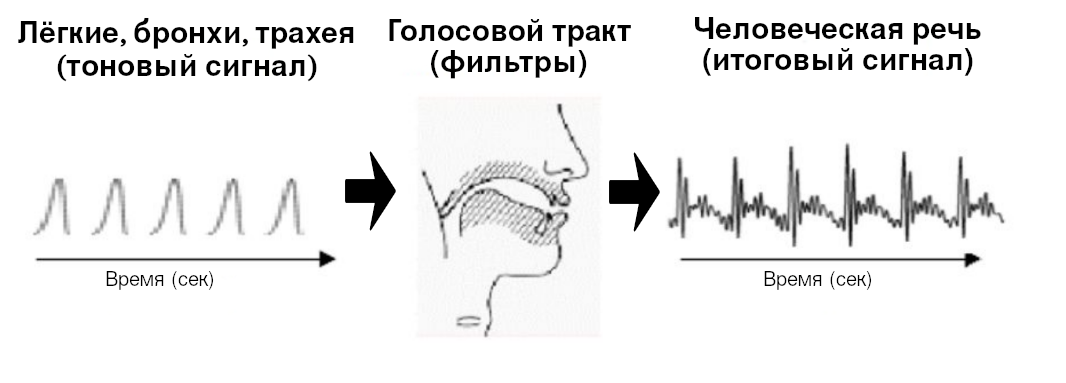
\includegraphics[scale=1.6]{speech_components.png}\]
	\caption{Речеобразование}
	\label{fig:speech_components}
\end{figure}

Распознавание речи происходит на основе анализа определённых признаков, которые причастны определенным звукам. За создание этих особенностей отвечает голосовой тракт человека. Поэтому одной из подзадач предобработки звука является выделение той части сигнала, которая была сформирована именно голосовым трактом.

Произнесённая речь поступает в приёмники звука. В случае человеческого уха происходит следующее. Звуковые волны проходят через наружное ухо в среднее и вызывают вибрацию барабанной перепонки. Колебания с барабанной перепонки передаются на маленькие слуховые косточки в среднем ухе. А со слуховых косточек — во внутреннее ухо. Когда эти колебания достигают улитки, они воздействуют на специальные клетки — волосковые. Волосковые клетки преобразуют колебания в электрические нервные импульсы. Слуховой нерв соединяет улитку с центрами слуха в головном мозге. Когда электрические нервные импульсы достигают головного мозга, они воспринимаются как звук и обрабатываются.

В случае с компьютером и подключённым к нему микрофоном - принцип схожий. Звуковые волны колеблют мембрану в микрофоне. Разница в положении мембраны замеряется в виде электрического сигнала при помощи, например, конденсатора.  Далее электрический сигнал, поступает по проводу в компьютер, и там проходит обработку.

Речь можно представить в виде последовательности предложений, а их в свою очередь в виде последовательности слов. Слова же состоят из фонем. В общем случае речь непрерывна, т.е. слова не отделяются друг от друга паузами, за исключением того требующих пунктуационных особенностей. В этой работе не рассматривается общий случай. Здесь рассмотрен частный случай, когда речь состоит из отдельных слов, отделяемых друг от друга тишиной в понимании человеческой речи. Этот выбор был обусловлен командным типом системы распознавания, которая работает с отдельными словами.

\subsection{Речь в компьютерном представлении}
Каждая речевая команда с точки зрения звуковой записи в компьютере - это набор амплитудных значений, полученных с микрофона и записанных в звуковой файл.

\subsection{Общая схема алгоритма распознавания}
На рисунке \ref{fig:algo_scheme} представлена общая схема работы алгоритма распознавания речевых команд. Алгоритм разделен на два основных блока, обозначенных на рисунке как Блок 1 и Блок 2. На вход алгоритму поступает наборы амплитудных значений и соответствующие частоты дискретизации в формате wav. На выходе алгоритма - текстовое представление команды.

\begin{itemize}[leftmargin=2cm]
\item Блок 1 - блок, отвечающий за первоначальную обработку данных и приведение их к единому формату. 
\item Блок 2 - блок, отвечающий за классификацию унифицированных данных. Этот блок может работать в двух режимах: обучения и непосредственной работы. В режиме обучения меняются параметры алгоритма, которые влияют на конечный результат. В режиме непосредственной работы этого не происходит.
\end{itemize}


\begin{figure}[H]
  \[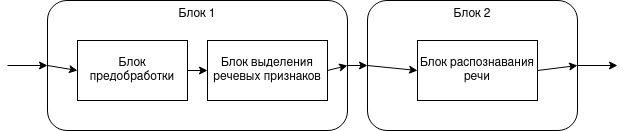
\includegraphics[scale=0.6]{algo_scheme.png}\]
  \caption{Общая схема работы алгоритма распознавания речевых команд}
  \label{fig:algo_scheme}
\end{figure}
